% IMPORTANT: PLEASE USE XeLaTeX FOR TYPESETTING
\documentclass{sintefbeamer}
\usepackage{xeCJK}
\usepackage{amsthm}
\setbeamertemplate{theorems}[numbered]
\makeatletter
\setbeamertemplate{footline}
{
  \leavevmode%
  \hbox{%
  \begin{beamercolorbox}[wd=.7\paperwidth,ht=2.25ex,dp=1ex,center]{title in head/foot}%
    \usebeamerfont{title in head/foot} {基于数据生成的类别均衡联邦学习}
  \end{beamercolorbox}%
  \begin{beamercolorbox}[wd=.3\paperwidth,ht=2.25ex,dp=1ex,right]{date in head/foot}%
    \usebeamerfont{date in head/foot}\insertshortdate{}\hspace*{2em}
    \insertframenumber{} / \inserttotalframenumber\hspace*{2ex} 
  \end{beamercolorbox}}%
  \vskip0pt%
}

%\newtheorem{theorem}{Theorem} % to number according to section
\theoremstyle{definition}

\makeatother

% meta-data
\title{\huge 基于数据生成的类别均衡联邦学习}
\subtitle{汇报人:黄其涵 \qquad 导师:章静 教授 \qquad }
\author{计算机学报, 2023}
\date{\today}
\titlebackground{images/bg4}

% document body
\begin{document}

\maketitle


\section{研究背景}{}

\begin{frame}{1.1 联邦学习}
\begin{itemize}
\item 联邦学习是一种分布式机器学习方法,其利用一个中央服务器(也称为服务器端)协调各终端设备(也称为客户端),协同训练一个各客户端共享的全局模型。

\item 与传统中心化训练方法不同,\textbf{联邦学习不需要各设备发送自身隐私数据至数据中心,因此有利于保护数据隐私。}具体而言,联邦学习在客户端和服务器端之间通过多轮通信迭代优化模型。
\item 每轮通信包含两个阶段:
\begin{itemize}
\item[(1)]各客户端从服务器端下载全局模型,并在本地数据上进行训练以获得本地模型;
\item[(2)]服务器端接收并聚合各客户端的本地模型参数以获得性能更优的全局模型.然而,现有联邦学习机制尚面临两大不足。
\end{itemize}
\end{itemize}



\end{frame}

\begin{frame}{1.2 现有问题}
\begin{columns}
\begin{column}{0.45\textwidth}
\begin{figure}[ht]
\centering
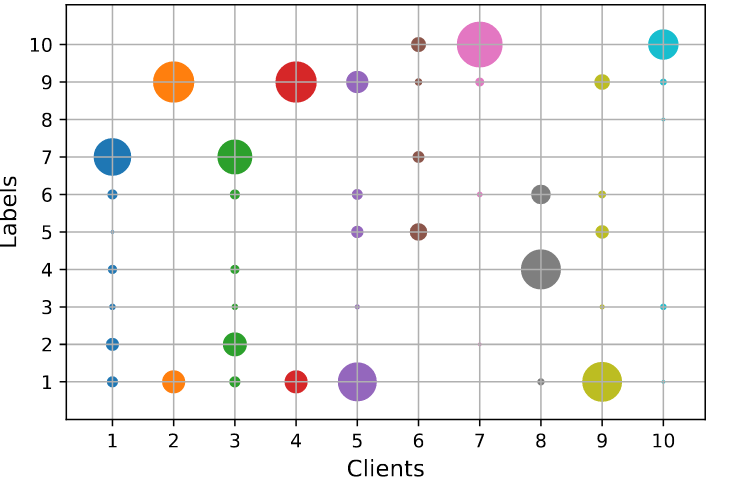
\includegraphics[width=1\textwidth]{images/img_unbalance}
\end{figure}
\end{column}
\begin{column}{0.65\textwidth}
\begin{itemize}
\item \textbf{类别不均衡。}全局模型需考虑多个客户端的数据,但各客户端往往仅包含部分类别数据且类别间数据量严重不均衡,使得全局模型难以训练。所训练的本地模型容易过拟合本地数据而在全局数据上往往取得较差性能。更重要的是,这些性能较差的本地模型严重影响全局模型的训练,导致难以构建高性能全局模型。
\item \textbf{数据分布差异。}由于各客户端的功能和用户使用习惯不同,不同客户端往往产生不同类别的数据,导致各客户端数据之间的类别分布差异较大。
\end{itemize}
\end{column}
\end{columns}
\end{frame}


\begin{frame}{1.3 主要贡献}
\begin{itemize}
\item \textbf{本文提出类别分布均衡器来均衡客户终端的类别分布。}其中,类别分布均衡器由类别均衡采集样器和数据生成器组成。类别均衡采样器对客户端数据量不足的类别以较高概率进行采样,数据生成器则根据所采样的类别生成相应的虚拟数据;
\item \textbf{基于类别分布均衡器,本文提出一种新颖的类别均衡联邦学习方法(CBFL)。}CBFL在客户端构造类别均衡的数据集进行训练,从而提高各本地模型的性能并减少各本地模型之间的差异性,进而构建高性能全局模型;
\item \textbf{本文在四个标准数据集上进行了大量实验,证明了所提出CBFL的有效性.}与最新方法相比,CBFL在多种深度神经网络(如ResNet20和MobileNetV2)取得更优越的性能.尤其在客户端上类别分布高度不均衡且客户端之间类别分布差异巨大的情况下,CBFL比现有方法具有更大的优势.
\end{itemize}
\end{frame}

\section{问题定义}

\begin{frame}{2 优化目标}

\begin{columns}
\begin{column}{0.4\textwidth}
\begin{figure}[ht]
\centering
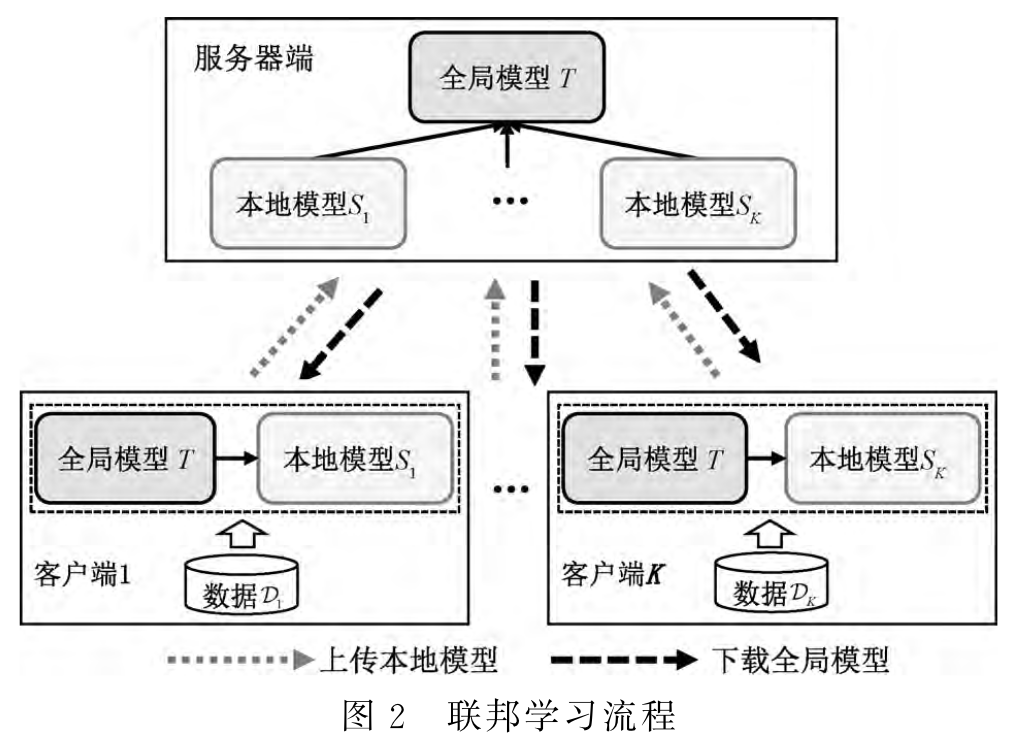
\includegraphics[width=1\textwidth]{images/img_fl}
\end{figure}
\end{column}
\begin{column}{0.6\textwidth}
为解决上述难题, 本文提出在客户端构造类别均衡的数据集进行训练的策略。 令 $\mathcal{D}$ 表示所构造的类别 均衡数 据集, $M$ 表示全局数据的类别数,则 $\mathcal{D}=\left\{(x, y) \mid P(y=i)=\frac{1}{M}, \quad i \in\{0,1, \ldots, M-1\}\right.$.
$p(\mathcal{D})$ 表示数据集 $\mathcal{D}$ 所代表的经验分布. 因此, 本文 旨在解决如下优化问题:
$$
\min _{\boldsymbol{W}_T} \mathbb{E}_k\left[\mathbb{E}_{x_k \sim p(\mathcal{D})}\left[\mathcal{L}\left(x_k ; \boldsymbol{W}_T\right)\right]\right]
$$
与仅仅利用客户端本地数据进行训练的方式相比,基于类别均衡的数据集进行训练使得各客户端本地模型之间的差异大大减少。
\end{column}
\end{columns}


\end{frame}

\section{研究方法}

\begin{frame}{3.1 CBFL方案框架}
\centering
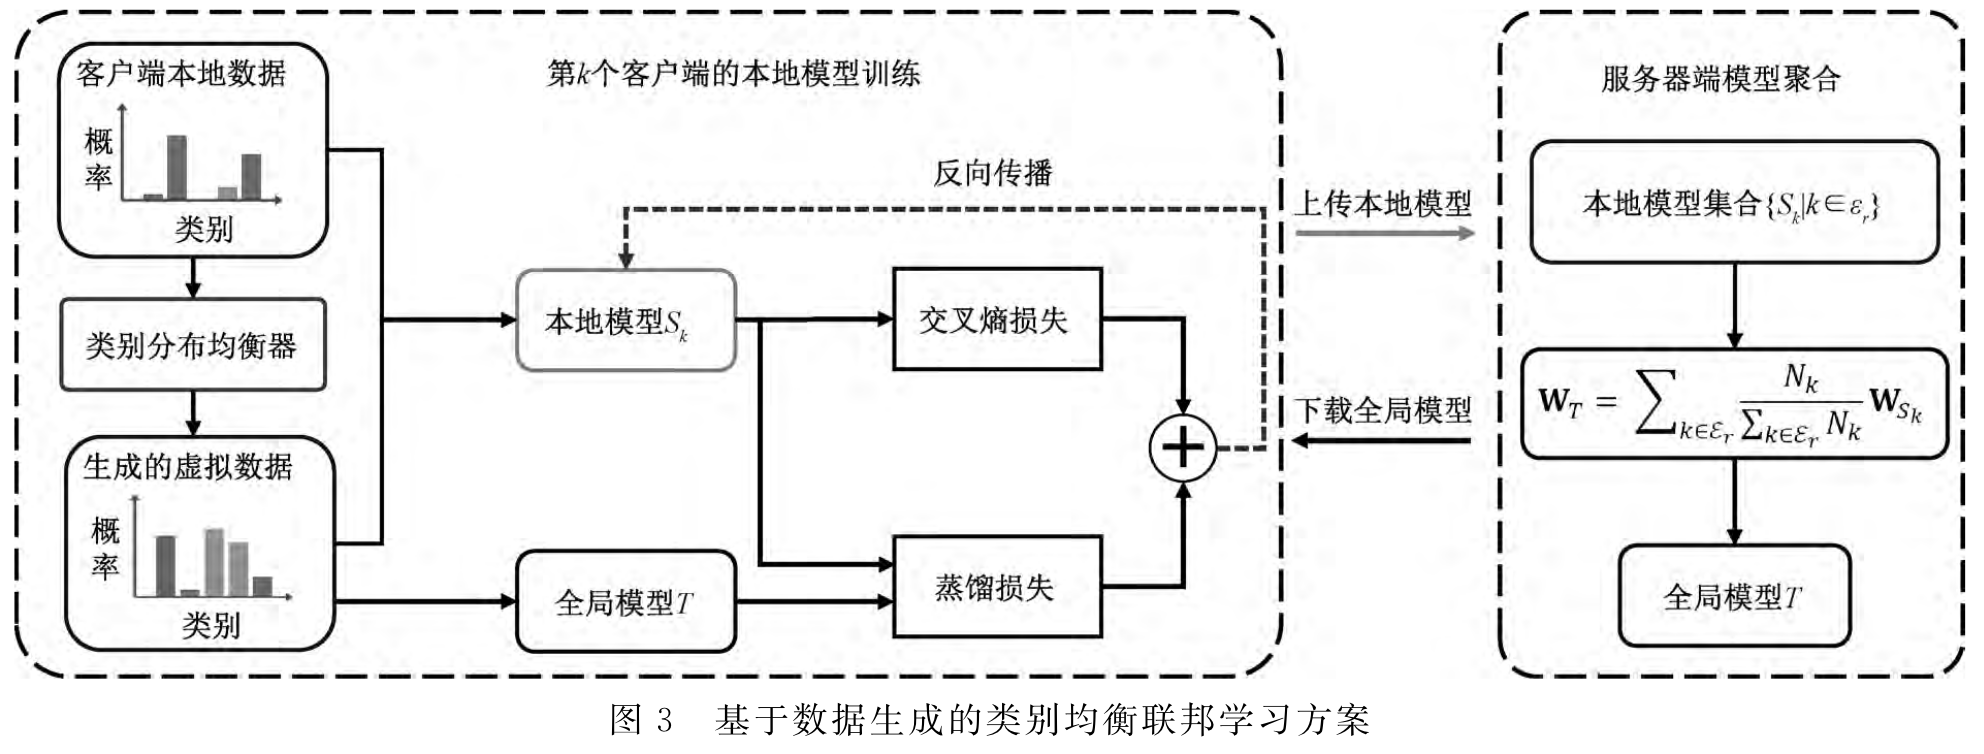
\includegraphics[width=1\textwidth]{images/img_overview}

\end{frame}

\begin{frame}{3.2 数据生成方案}
\centering
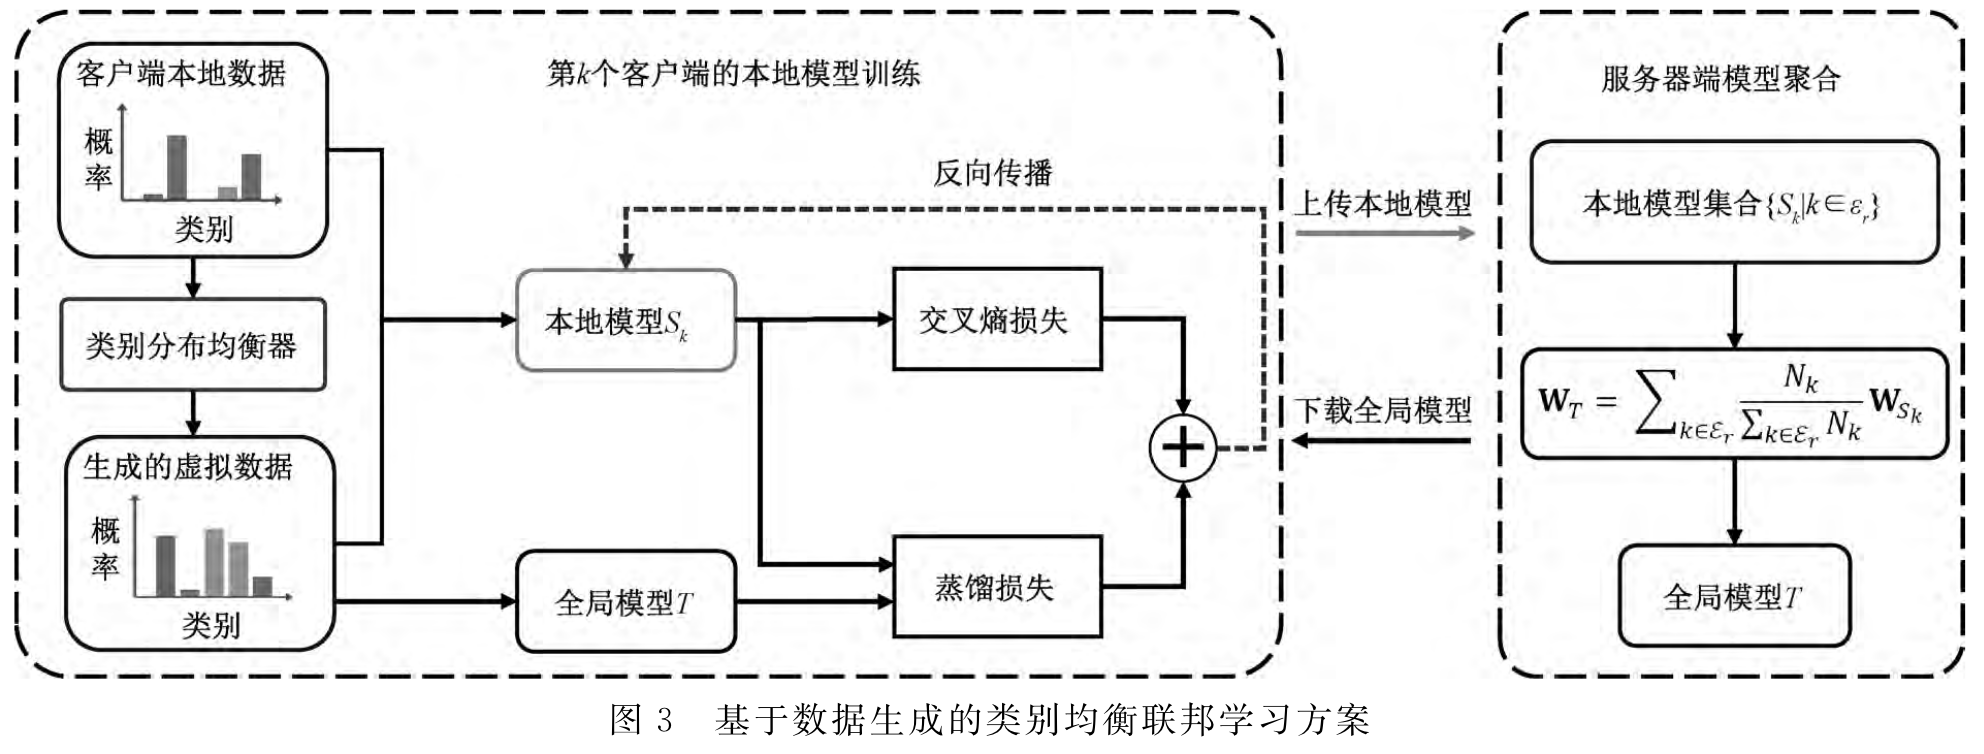
\includegraphics[width=1\textwidth]{images/img_overview}

\end{frame}

\begin{frame}{3.2 Committee Mechanism}{Scoring System}
评分系统的关键是通过计算欧氏距离来区分诚实梯度和恶意梯度。两个诚实梯度的欧氏距离低于诚实梯度和恶意梯度的欧氏距离。基于这种认识,评分系统被设计为比较两个梯度的欧氏距离,其中上传诚实梯度的客户端可以获得更高的分数,而上传恶意梯度的客户端将获得较低的分数。
\\ \hspace*{\fill} \\
Assume that the local gradient on the $k$-th training client at round $t$ is denoted as $\hat{g}_k^t=g_k\left(\mathbf{w}_{k, \tau}^t, \mathcal{B}_{k, \tau}^t\right)$, and the local gradient on the the $c$-th committee client at round $t$ is expressed as $\hat{g}_c^t=g_c\left(\mathbf{w}_{c, \tau}^t, \mathcal{B}_{k, \tau}^t\right)$. The score $\mathcal{P}_k^c$ of the $k$ th training client assigned by the $c$-th committee client is computed as follows:
$$
\mathcal{P}_k^c=\frac{1}{\left\|\hat{g}_k^t-\hat{g}_c^t\right\|_2^2} .
$$
\end{frame}

\begin{frame}{3.2 Committee Mechanism}{Scoring System}
Since $\hat{g}_k^t$ and $\hat{g}_c^t$ are local gradients generated from different clients, we assume that $\hat{g}_k^t \neq \hat{g}_c^t$ for any $k \in S_b^t, c \in S_c^t$. We define 
$$
\mathcal{P}_k=\frac{1}{\frac{1}{C} \sum_c^C\left\|\hat{g}_k^t-\hat{g}_c^t\right\|_2^2}=\frac{C}{\sum_c^C \frac{1}{\mathcal{P}_k^c}}
$$
as the final score of the $k$-th training client. 
\\ \hspace*{\fill} \\
拜占庭攻击通常带有恶意梯度,这直接增加了这些梯度与诚实梯度之间的欧氏距离。因此,当恶意客户端的比例在可容忍范围内时,恶意训练客户端的分数预计会低于诚实训练客户端。但是,在没有拜占庭攻击的情况下,分数代表客户端的异构程度。得分越高意味着异质性程度越高。
\end{frame}

\begin{frame}{3.2 Committee Mechanism}{Selection Strategy}
基于上述 Scoring System 可以通过接受高分梯度来实现安全聚合,因为恶意梯度会获得低分。此外,收敛分析和实验结果表明,相反的策略在非攻击场景中表现更好。因此,针对不同的考虑,本文还设计了两种相反的选择策略如下:
\begin{itemize}
\item Selection Strategy I. 选择几个得分相对较高的局部梯度来构建全局梯度,用于全局模型的更新。此策略希望在欧几里德空间中类似于委员会梯度的局部梯度参与全局梯度的构建。
\item Selection Strategy II. 选择几个得分相对较低的局部梯度来构建全局梯度,用于全局模型的更新。此策略希望欧几里德空间中不同于委员会梯度的局部梯度参与全局梯度的构建。
\end{itemize}
\end{frame}

\begin{frame}{3.2 Committee Mechanism}{Election Strategy}
Election Strategy 旨在保证委员会客户的诚实。因此,委员会必须保证诚实的成员多于恶意的成员。否则,委员会无法过滤掉恶意梯度。本文根据分数对训练成员进行排序,然后选择这些靠近中间位置的训练成员作为下一轮的委员会成员。本文基于以下两个方面考虑来设计选举机制:
\begin{itemize}
\item \textbf{Robustness. } 恶意训练客户端会比诚实训练客户端获得更低的分数。因此,选择靠近中上位的训练客户端,可以防止恶意训练客户端成为下一轮的委员会客户端,从而保证全局模型的安全性。
\item \textbf{System Stability. } 得分最高的培训客户不会被选为新的委员会成员,以避免系统过于依赖委员会成员的初始化。即应符合“委员应该是能代表多数的人”的直觉。
%当我们选择那些得分最高的训练客户组成新的委员会时,全局模型的学习方向将完全由初始委员会成员决定。这是因为那些局部梯度与委员会梯度之间欧氏距离较大的客户,不仅难以被选中参与聚合过程,而且失去了竞选下一轮委员会成员的机会。这符合我们“委员应该是能代表多数的人”的直觉。
\end{itemize}


\end{frame}








\section{实验分析}

\begin{frame}{4.1 数据集}

	\begin{itemize}
\item[1)] CIFAR-10由60000张32×32像素的彩色图像组成,共包含10个类别,每个类别包含6000张图像.训练集与测试集分别包含50000张和10000张图像; 
\item[2)] CIFAR-100与CIFAR-10的组成相似,但CIFAR-100包含了更多的类别.CIFAR-100共包含100个类别,每个类别包含500张训练图像和100张测试图像; 
\item[3)] CINIC-10包含270000张图像.值得一提的是,该数据集的图像不一定来自相同的分布.这个特性非常适合联邦学习,因为实际场景中各个客户端的数据不一定服从相同分布.CINIC-10具有相同大小的训练集、验证集和测试集.本文在训练集上进行模型训练,并在测试集上进行测试,而不使用该数据集的验证集; 
\item[4)] iNaturalist2019是一个大规模的类别分布高度不均衡的真实数据集.该数据集包含1010个类别,总计268243张彩色图片,由i Naturalist网站的2295个用户收集和上传.每个用户上传的图片被视为一个客户端的数据集.
\end{itemize}
\end{frame}

\begin{frame}{4.2 对比模型}
	本文将CBFL与目前最新的方法进行比较,即FedAvg、FedPoxr、SCAFFOLD和FedNvao.本实验通过狄利克雷分布Dir(0.1)模拟各客户端数据的类别分布.所有方法基于两种常见的深度神经网络模型(即ResNet20和MobileNet V2)进行训练和性能比较.
\end{frame}


\begin{frame}{4.3 实验结果}{Result Analysis}
	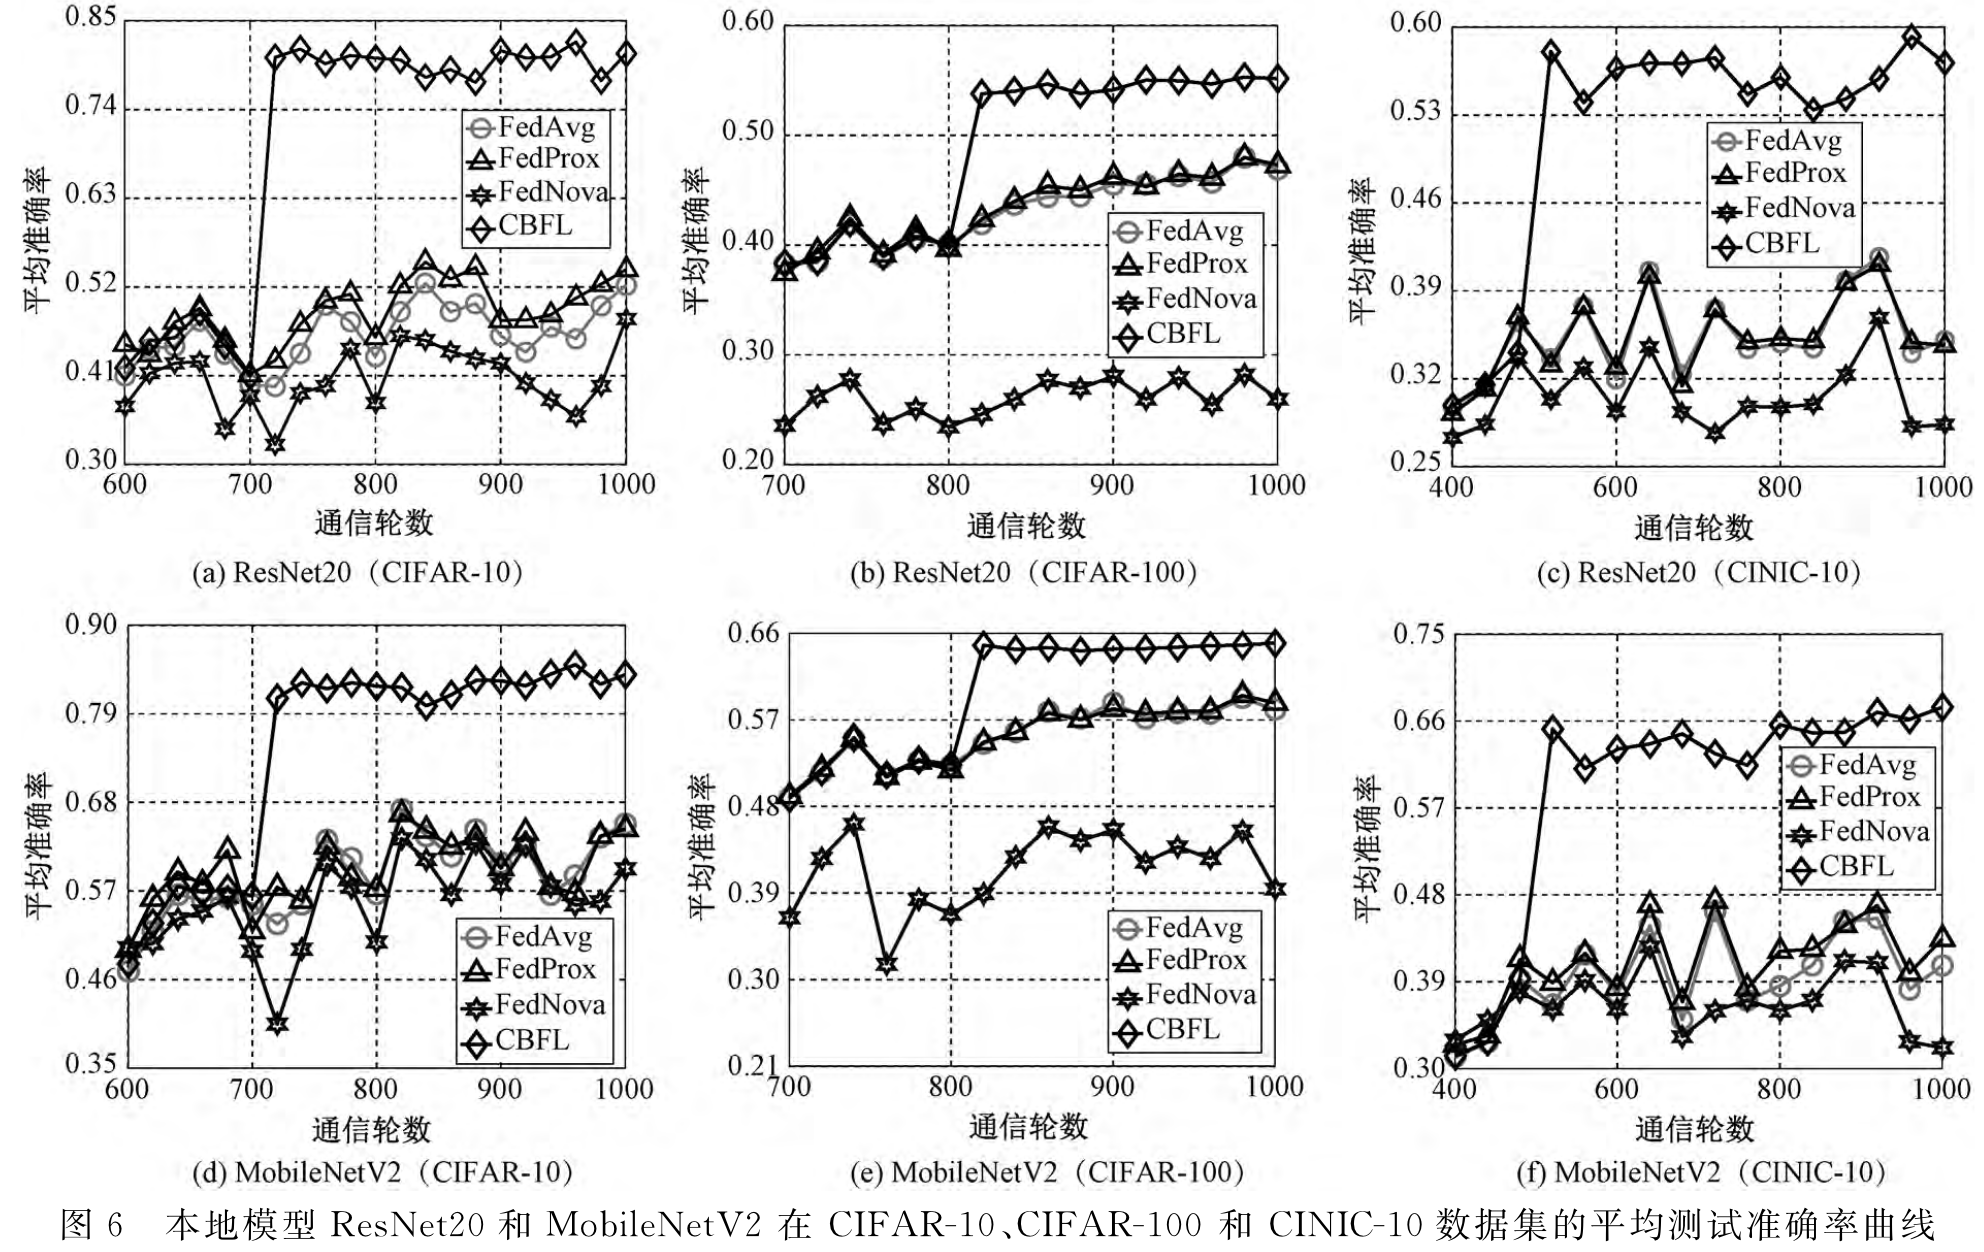
\includegraphics[width=0.75\textwidth]{images/img_expr1}
\end{frame}

\begin{frame}{4.3 实验结果}{Result Analysis}
	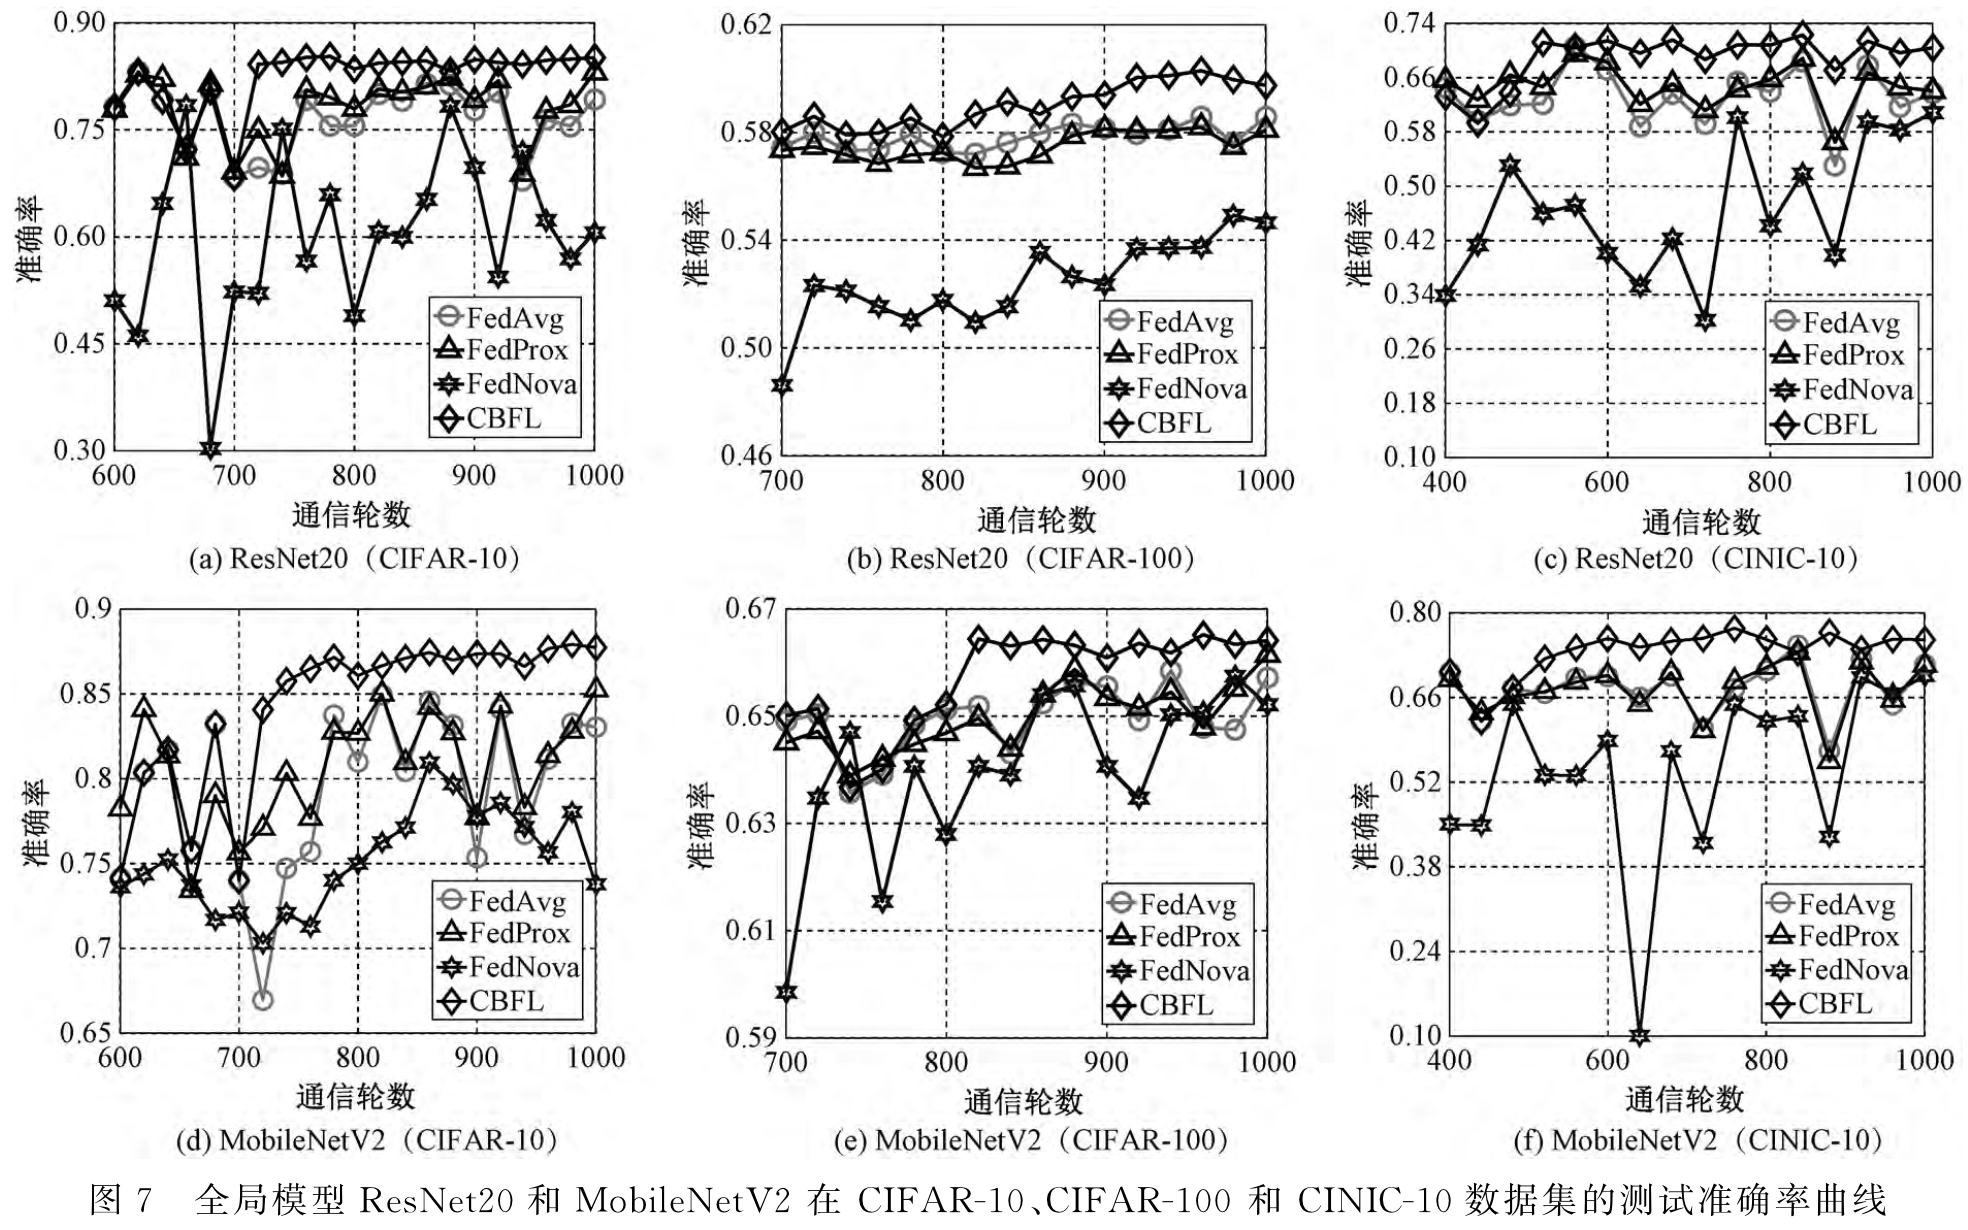
\includegraphics[width=0.75\textwidth]{images/img_expr3}
\end{frame}

\begin{frame}{4.3 实验结果}{Result Analysis}
	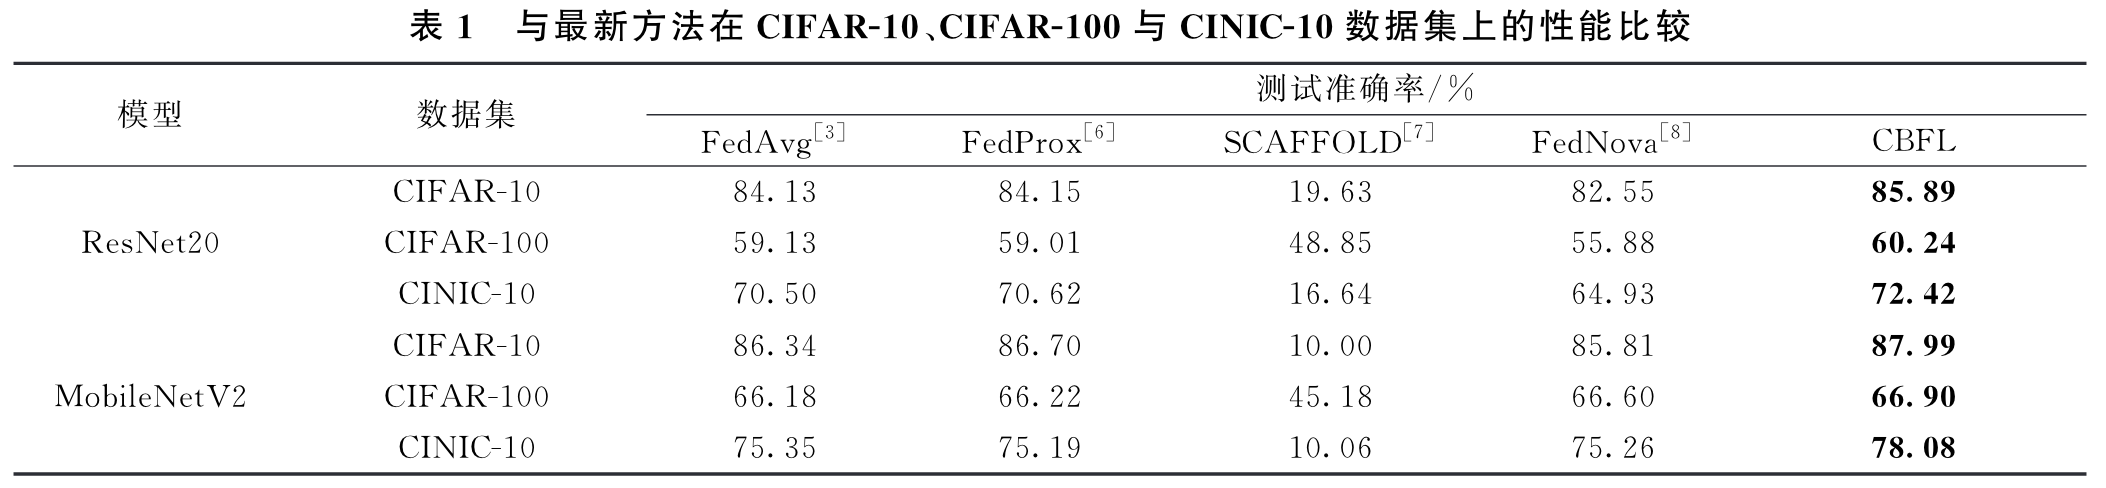
\includegraphics[width=1.\textwidth]{images/img_expr2}
\end{frame}

\begin{frame}{4.3 实验结果}{Result Analysis}
	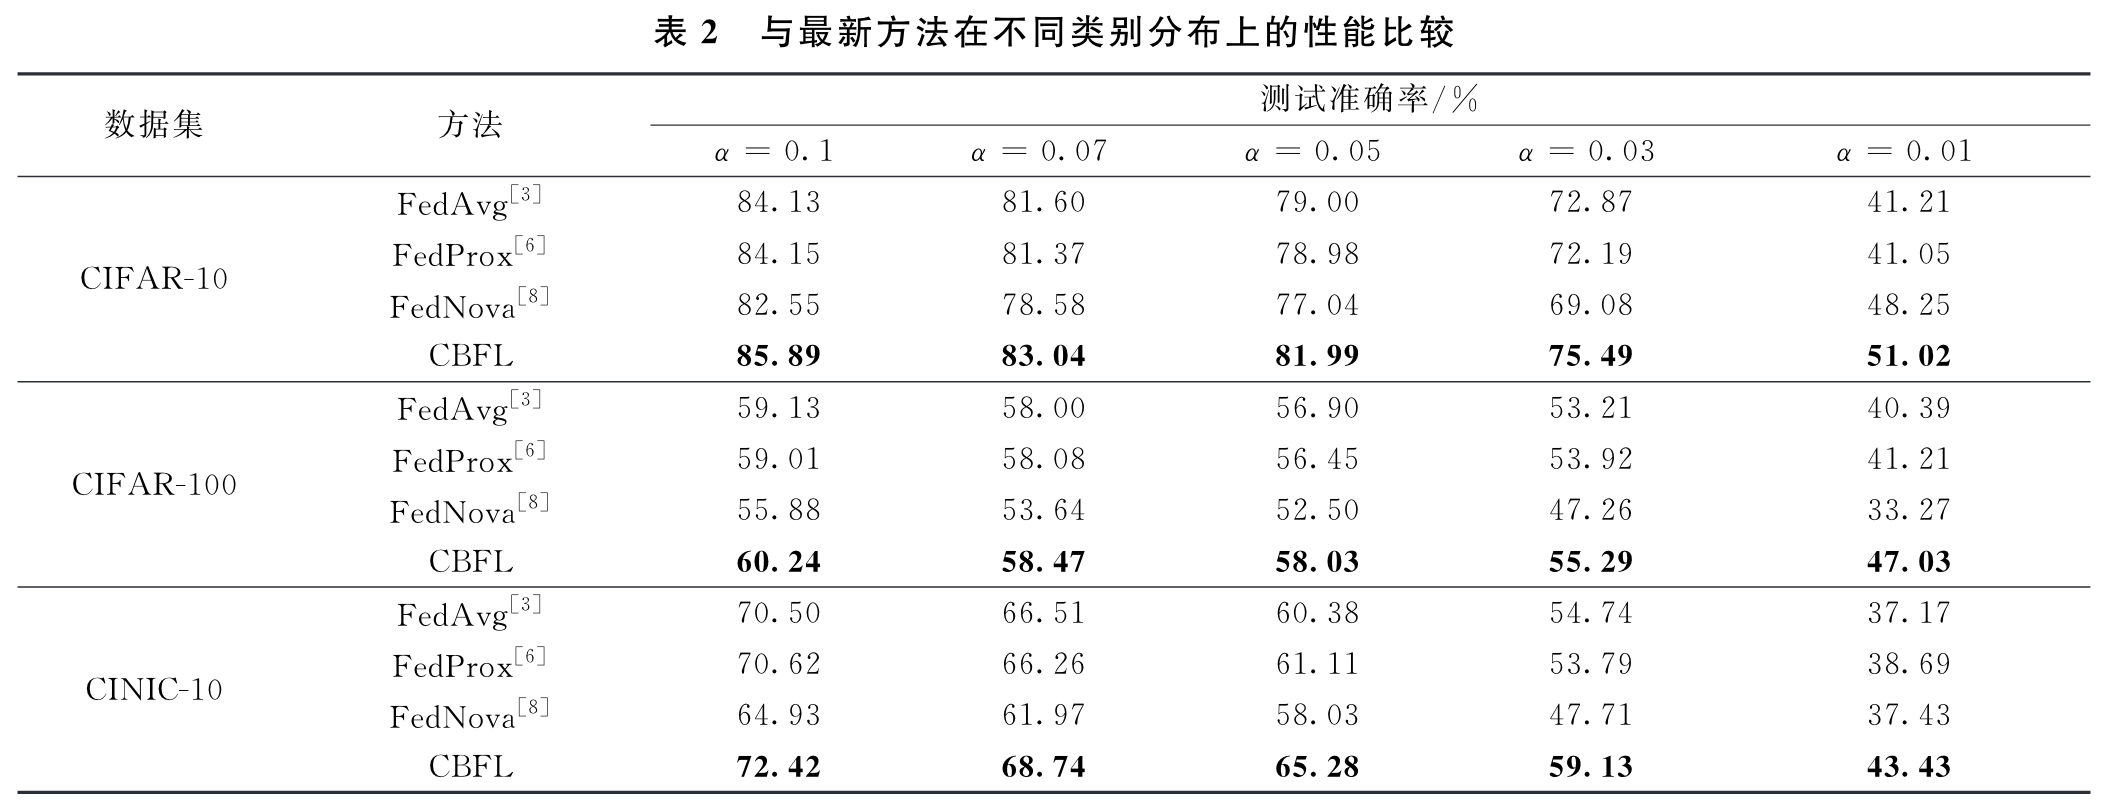
\includegraphics[width=1.\textwidth]{images/img_expr4}
\end{frame}



\section{研究总结}

\begin{frame}{研究总结}

本文提出了一种基于数据生成的类别均衡联邦学习(CBFL)方法.CBFL针对各客户端构造类别均衡的数据集,以降低客户端类别不均衡和客户端之间分布差异的影响.
\\ \hspace*{\fill} \\
具体而言,CBFL设计了一个类别分布均衡器,其由一个类别均衡采样器和一个数据生成器组成.其中,类别均衡采样器以较高概率采样客户端本地数据量不足的类别,然后,数据生成器根据所采样的类别生成相应的虚拟数据.结合本地数据和虚拟数据,客户端构造类别均衡的数据集来进行模型训练,从而有利于构建高性能全局模型.
\end{frame}



\backmatter

\end{document}
